\chapter{Sistemas de Reconhecimento Automático de Voz}

Sistemas de reconhecimento automático de voz, tem como objetivo, transformar um sinal analógico(fala) obtido através de um transdutor \footnote{Dispositivo que transforma um tipo de energia em outro, utilizando para isso um elemento sensor}, mapeando-o a fim de produzir como saída a palavra, uma sequencia de fonemas ou uma sentenças correspondentes ao sinal de entrada. Com o resultado da tradução, pode-se tomar decisões, traduzir para outra língua, etc.

%Descobrir o q eh analógico digital
A primeira etapa é a \textit{aquisição de voz}, processo pelo qual ondas sonoras são convertidas em sinais elétricos, e depois é feita uma conversão analógico-digital do mesmo. Algumas características do ambiente de gravação podem atrapalhar no processo de reconhecimento, como ruídos, distância do microfone, etc. Assim é preciso passar por uma fase que é feita uma filtragem afim de tornar o sinal o mais próximo possível da fala pura, o nome desta etapa é \textit{Pré-Processamento}. Logo depois, é feita a \textit{extração de informações} do sinal, que consiste em representar segmentos, fonemas ou qualquer outra unidade de fala com o menor número possível de parâmetros, de forma que estes contenham informações suficientes para caracterizar o sinal de fala, já que um sinal digital possui uma grande quatidade de parâmetros, então a exigência por tempo e processamento seriam muito altas. Outra etapa, e uma das mais importantes é a \textit{geração de padrões}, também chamada de padrões de referência, que é realizada durante o treinamento do sistema, nesta fase é gravado o maior número possível de padrões, para cada palavra cadastrada no dicionário, para garantir o melhor funcionamento e tempo de resposta do reconhecedor.
\cite{RavIsolAnderson}, \cite{RavComputLouzada}. 


\section{Fala}
A fala é a forma de comunicação mais utilizada pelos seres humanos \cite{RavCorporaCarlos}. Através da fala, o cérebro humano consegue interpretar informações extremamente complexas, tais como identificar a pessoa que está falando, sua posição no espaço físico, seu estado emocional e outros dados como a ironia, seriedade ou tristeza. Os computadores, apesar de fazerem cálculos mais rápidos que o homem, não conseguem reconhecer através da fala informações como os seres humanos.

\subsubsection{Vantagens da comunicação pela fala em sistemas homém-máquina}

Segundo \citeonline{RavDigitalSadaoki} podemos citar:

\begin{itemize}
\item Naturalidade: Não precisa de treinamento especial e nem de habilidades especiais;
\item Rapidez: A informação é transmitida mais rapidamente que pelas outras formas de comunicação.
\item Flexibilidade: Deixa as mãos, olhos livres;
\item Eficiência: Tem uma elevada taxa de informação;
\end{itemize}

\subsubsection{Desvantagens no uso da fala em sistemas homem-máquina}
Mesmo possuindo vantagens significativas, a comunicação por fala também possui desvantagens, como \citeonline{RavDigitalSadaoki} descreveu:

\begin{itemize}
\item Ruidos: O sistema fica suscetível a interferência do ambiente, necessitando de um removedor de ruídos para ambientes com alto índice de ruídos.
\item Diversidade da língua: Características que variam de pessoa para pessoa, como sotaque, velocidade da fala, condições físicas e emocionais do locutor. 
\end{itemize}
%Tentar procurar mais desvantanges e argumentos para diversidade.

\subsection{Aquisição do sinal de fala}
Aquisição do sinal de fala é a primeira etapa de um sistema \textit{RAV}, ele é responsável por capturar e converter um sinal analógico em um sinal elétrico, esse processo pode ser feito através de um microfone ou telefone. Todas as etapas de aquisição de voz, podem ser vistas na figura 1 \cite{RavIsolAnderson}:

\begin{figure}
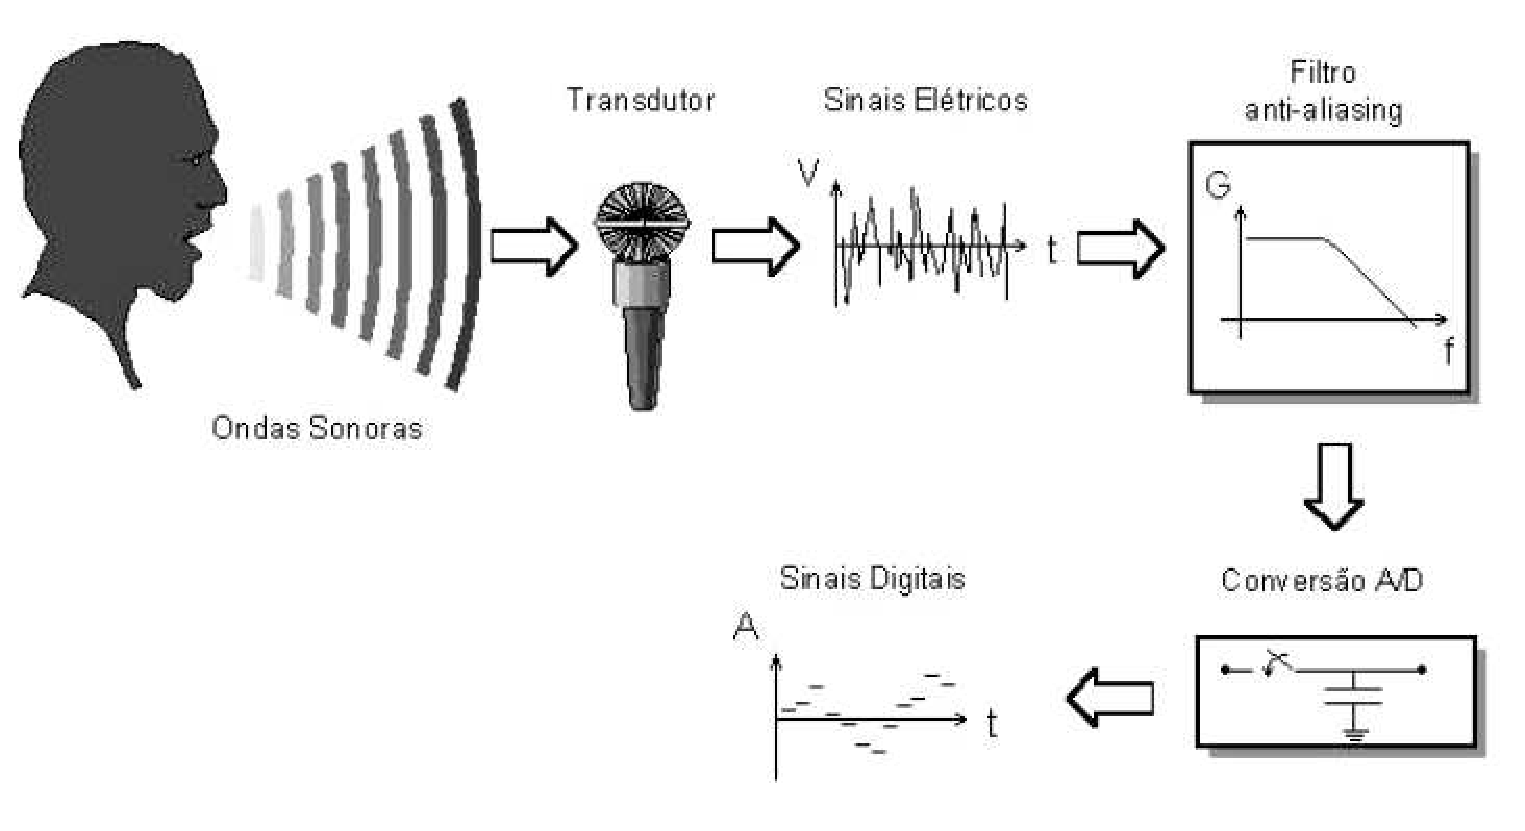
\includegraphics[width=1\textwidth]{graficos/aquisicao_fala.eps}
\caption{Processo de aquisição do sinal da fala}
\end{figure}


\section{O Sistema de Reconhecimento de Voz}\label{sec:red_khn}

Sistemas de reconhecimento automático de voz vem sendo estudados desde os anos 50 nos laboratórios Bell, quando foi criado, o primeiro reconhecedor de dígitos isolados com suporte a um locutor \cite{MetodosProAnderson}. As redes neurais também surgiram nos anos 50, mas não houve prosseguimento nos estudos, devido a problemas práticos. Muitos reconhecedores de voz, foram criados nas décadas de 50 e 60 \cite{RavSpeechSadaoki}. \citeonline{FundamentRabiner} mostra que no início dos anos 70, surgiram os algoritmos para sistemas de fala contínua, graças as técnicas de \textit{Linear Predictive Coding} (LPC) e \textit{Dynamic Time Warping} (DTW). E os anos 80 foram marcados pela disseminação dos metodos estáticos, como \textit Modelos Ocultos de Markov (HMM). Esse período foi de grande evolução para os sistemas de reconhecimento de voz, as redes neurais passaram a ser usadas no desenvolvimento dos sistemas, sendo possível implementar sistemas mais robustos, com vocabulários grandes e com taxas de acerto de mais de 90{\%} \cite{AvaliaTecJose}.
\citeonline{FundamentRabiner} classifica os reconhecedores de voz em três grandes classes: \textit{reconhecimento por comparação de padrões}, \textit{reconhecimento baseado na análise acústico-fonética} e \textit{reconhecimento empregando inteligência artificial}. No reconhecimento por comparação de padrões, existem duas formas distintas: treinamento e reconhecimento. Na fase de treinamento, são apresentados padrões ao sistema para criação de representantes, para cada um dos padrões. A fase de reconhecimento compara um padrão ainda desconhecido, com os padrões existentes no sistema, o que mais se aproximar do padrão existente, é escolhido como o padrão reconhecido. A fase de treinamento é fundamental para o sucesso do sistema, portanto uma quantidade considerável de material será necessário para a fase de treinamento. 

Sistemas com Modelos Ocultos de Markov (HMM) utilizam essa classe de reconhecimento \cite{AvaliaTecJose}. Nos sistemas com reconhecimento baseado na análise acústico-fonema, o sinal de fala é decodificado baseado em suas características acústicas e nas relações entre essas características \cite{DigSpeechNejat}. É identificada as unidades fonéticas da fala a ser reconhecida, e concatenando essas unidades é reconhecida a palavra. Nessa análise é necessário considerar as propriedades invariantes da fala. Segundo \citeonline{AvaliaTecJose} Um analisador acústico-fonética apresenta as sequintes fases: análise espectral, detecção das características que descrevem as unidades fonéticas, a fase mais importante de todo o processo que é: segmentação do sinal de fala e identificação das unidades fonéticas e escolha da palavra que melhor corresponde a sequência de unidades. 

Reconhecimento empregando inteligência artificial explora os conceitos tanto do reconhecimento por padrões quanto o baseado em análise acústico-fonema. Utilizando redes neurais, cria-se uma matriz de ponderações que representa os nós das redes, e suas saídas, estão relacionadas as unidades a serem reconhecidas \cite{AvaliaTecJose}.
O processo para o reconhecimento de voz pode ser dividido em quatro fases: aquisição do sinal de voz, pré-processamento, extração de informações e geração dos padrões de voz \cite{RavIsolAnderson}.

\begin{figure}[H]
\centering
% Generated with LaTeXDraw 2.0.8
% Thu Mar 15 10:13:30 BRT 2012
% \usepackage[usenames,dvipsnames]{pstricks}
% \usepackage{epsfig}
% \usepackage{pst-grad} % For gradients
% \usepackage{pst-plot} % For axes
\scalebox{0.7} % Change this value to rescale the drawing.
{
\begin{pspicture}(0,-2.64)(23.98,2.66)
\psline[linewidth=0.04cm,arrowsize=0.05291667cm 2.0,arrowlength=1.4,arrowinset=0.4]{->}(0.0,0.6)(1.58,0.58)
\psframe[linewidth=0.04,dimen=outer](4.4,1.44)(1.58,-0.3)
\psline[linewidth=0.04cm,arrowsize=0.05291667cm 2.0,arrowlength=1.4,arrowinset=0.4]{->}(4.4,0.6)(5.98,0.58)
\psframe[linewidth=0.04,dimen=outer](8.82,1.48)(6.0,-0.26)
\psline[linewidth=0.04cm,arrowsize=0.05291667cm 2.0,arrowlength=1.4,arrowinset=0.4]{->}(8.84,0.62)(10.42,0.6)
\psframe[linewidth=0.04,dimen=outer](13.28,1.44)(10.46,-0.3)
\usefont{T1}{ppl}{m}{n}
\rput(0.70625,0.83){Fala}
\usefont{T1}{ppl}{m}{n}
\rput(2.9889061,0.91){Aquisição do}
\usefont{T1}{ppl}{m}{n}
\rput(2.9848437,0.33){Sinal de Voz}
\usefont{T1}{ppl}{m}{n}
\rput(7.382656,0.33){Processamento}
\usefont{T1}{ppl}{m}{n}
\rput(7.4384375,0.91){Pré-}
\usefont{T1}{ppl}{m}{n}
\rput(11.863438,0.85){Extração de}
\usefont{T1}{ppl}{m}{n}
\rput(11.867344,0.33){Informações}
\psframe[linewidth=0.04,dimen=outer](19.54,2.66)(16.72,0.92)
\psline[linewidth=0.04cm,arrowsize=0.05291667cm 2.0,arrowlength=1.4,arrowinset=0.4]{->}(14.2,0.6)(15.12,1.82)
\psline[linewidth=0.04cm](13.28,0.62)(14.24,0.62)
\psline[linewidth=0.04cm,dotsize=0.07055555cm 2.0]{oo-}(15.08,1.8)(16.72,1.8)
\usefont{T1}{ppl}{m}{n}
\rput(18.124844,2.01){Geração dos}
\usefont{T1}{ppl}{m}{n}
\rput(18.087343,1.49){Padrões}
\usefont{T1}{ppl}{m}{n}
\rput(15.470781,2.13){Treinamento}
\psframe[linewidth=0.04,dimen=outer](19.56,-0.86)(16.74,-2.6)
\psframe[linewidth=0.04,dimen=outer](23.98,-0.9)(21.16,-2.64)
\usefont{T1}{ppl}{m}{n}
\rput(18.150156,-1.73){Classificação}
\usefont{T1}{ppl}{m}{n}
\rput(22.46625,-1.51){Palavra}
\usefont{T1}{ppl}{m}{n}
\rput(22.53625,-2.09){Reconhecida}
\psline[linewidth=0.04cm,arrowsize=0.05291667cm 2.0,arrowlength=1.4,arrowinset=0.4]{->}(19.58,-1.76)(21.16,-1.78)
\psline[linewidth=0.04cm,dotsize=0.07055555cm 2.0]{oo-}(15.1,-1.76)(16.74,-1.76)
\usefont{T1}{ppl}{m}{n}
\rput(15.132656,-2.17){Reconhecimento}
\psarc[linewidth=0.04,arrowsize=0.05291667cm 2.0,arrowlength=1.4,arrowinset=0.4]{<-}(13.6,-0.48){2.18}{-29.890425}{74.5115}
\psline[linewidth=0.04cm,arrowsize=0.05291667cm 2.0,arrowlength=1.4,arrowinset=0.4]{cc->>}(18.14,0.94)(18.14,-0.9)
\end{pspicture} 
}


\caption{Diagrama de blocos de um sistema de reconhecimento de voz}
\end{figure}

%por padrões te simplicidade de uso, maior entendimento, boas justificativas matemáticas e robustez. AvaliaTecJose e FundamentRabiner






\subsection{Características de Sistemas RAV}\label{sec:red_neu}

Existem várias maneiras de categorizar um sistema de reconhecimento de voz, os mais importantes são: o estilo de pronuncia que é aceito, o tamanho do vocabulário e à dependência ou independencia do locutor \cite{RavIsolMartins}. Essas categorias que definem a precisão do sistema de reconhecimento:

\begin{enumerate}[(A)]
\item Dependência do locutor:

Podemos classificar sistemas de reconhecimento como dependentes e independentes do locutor. Um sistema dependente de locutor reconhece a fala das pessoas cujas vozes foram utilizadas para treinar o sistema, apresentando uma pequena taxa de erros, para o locutor para qual foi treinado o sistema,  implementação mais simples que sistemas independentes do locutor, que reconhecem a fala de qualquer pessoa com uma taxa de acerto aceitável. Neste caso é necessário realizar o treino do sistema com uma base que inclua diferentes pessoas com diferentes idades, sexo, sotaques, etc. O que dificulta a construção desses sistemas.
\item Modo de pronúncia:

%Pesquisar conectas e contínua para o caso de serem diferentes
Sistemas RAV podem ser classificados quanto ao modo de pronúncia de duas formas, sistemas de palavras isoladas e os de fala conectadas(contínua). Reconhecedor de palavras isoladas são sistemas que reconhecem palavras faladas isoladamente, isto é, entre cada palavra deve existir uma pausa mínima, para que seja detectado o início e o fim da mesma. Isso proporciona um resultado muito superior aos de fala contínua, estes sistemas são os mais simples de serem implementados. Um exemplo clássico de reconhecedores de palavras isoladas são os reconhecedores de dígitos, que segundo \citeonline{RavPtBrCarlos} alcançam taxa de menos de 2{\%} de erro para dígitos de 0 à 10.
Já o reconhecedor de palavras conectadas são sistemas mais complexos que os de palavras isoladas e utilizam palavras como unidade fonética padrão. São capazes de reconhecer sentenças completas, pronunciadas sem pausa entre as palavras, e por isso não se tem informação de onde começam e terminam determinadas palavras, muitas palavras são mascaradas, encurtadas e as vezes não pronunciadas. Esses sistemas precisam lidar com todas as características e vícios da linguagem natural, como o sotaque, a duração das palavras, a pronúncia descuidada, etc. Tornando ainda mais difíceis as tarefas do reconhecedor em casos como “ele vai morrer em dois dias” que 
muitas vezes  é dito como “ele vai morrerem dois dias”.
\item Tamanho do vocabulário:

Um fator muito importante na precisão de um RAV, é o tamanho do vocabulário, quanto maior seu tamanho, maior a quantidade de palavras ambíguas, com realizações sonoras semelhantes, ocasionando maior chance de erros por parte do decodificador responsável pelo reconhecimento. Segundo \cite{RavIsolAnderson} vocabulários podem ser definidos como:

\begin{itemize}
\item Vocabulário pequeno: reconhecem até 20 palavras. 
\item Vocabulário médio: reconhecem entre 20 e 100 palavras. 
\item Vocabulário grande: reconhecem entre 100 e 1000 palavras. 
\item Vocabulário muito grande: reconhecem mais de 1000 palavras. 
\end{itemize}

Sistemas RAV com suporte a grandes vocabulários são chamados de Large Vocabulary Continuos Speech Recognition (LVCSR). Existem muitas dificuldades encontradas na criação de sistemas LVCSR, como: a disponibilidade de um corpus de voz digitalizada e transcrita grande o suficiente para treinamento do sistema, recursos como bases de textos de
tamanho elevado e um dicionario fonético de amplo vocabulário.

%\item Perplexidade
%\item Relação snial - ruído

\end{enumerate}

\section{Reconhecimento de voz baseado em padrões}\label{sec:red_neu}
De acordo com \citeonline{AvaliaTecJose}, o reconhecimento baseado em padrões, é a técnica que oferece melhor resultado nos sistemas de reconhecimento de fala, então a implementação do sistema será usando essa técnica.
Um sistema de reconhecimento de voz usando reconhecimento de padrões poder ser representado na figura 2 \cite{FundamentRabiner}:
 
\begin{figure}[H]
\centering
% Generated with LaTeXDraw 2.0.8
% Wed Mar 14 21:20:50 BRT 2012
% \usepackage[usenames,dvipsnames]{pstricks}
% \usepackage{epsfig}
% \usepackage{pst-grad} % For gradients
% \usepackage{pst-plot} % For axes
\scalebox{0.8} % Change this value to rescale the drawing.
{
\begin{pspicture}(0,-2.51)(15.567813,2.51)
\psline[linewidth=0.04cm,arrowsize=0.05291667cm 2.0,arrowlength=1.4,arrowinset=0.4]{->}(0.0,-1.61)(1.58,-1.63)
\psframe[linewidth=0.04,dimen=outer](4.4,-0.77)(1.58,-2.51)
\psline[linewidth=0.04cm,arrowsize=0.05291667cm 2.0,arrowlength=1.4,arrowinset=0.4]{->}(4.4,-1.61)(5.98,-1.63)
\psframe[linewidth=0.04,dimen=outer](8.82,-0.73)(6.0,-2.47)
\psline[linewidth=0.04cm,arrowsize=0.05291667cm 2.0,arrowlength=1.4,arrowinset=0.4]{->}(8.84,-1.59)(10.42,-1.61)
\psframe[linewidth=0.04,dimen=outer](13.18,-0.75)(10.36,-2.49)
\usefont{T1}{ppl}{m}{n}
\rput(0.70625,-1.38){Fala}
\psframe[linewidth=0.04,dimen=outer](8.9,2.51)(6.08,0.77)
\psline[linewidth=0.04cm,arrowsize=0.05291667cm 2.0,arrowlength=1.4,arrowinset=0.4]{->}(7.5,0.79)(7.5,-0.77)
\usefont{T1}{ppl}{m}{n}
\rput(2.9426563,-1.12){Processamento}
\usefont{T1}{ppl}{m}{n}
\rput(2.943125,-1.66){do sinal}
\usefont{T1}{ppl}{m}{n}
\rput(2.9139063,-2.1){de Fala}
\usefont{T1}{ptm}{m}{n}
\rput(7.447344,2.1){Padrões}
\usefont{T1}{ptm}{m}{n}
\rput(7.367344,-2.08){Padrões}
\usefont{T1}{ptm}{m}{n}
\rput(7.521094,1.66){de}
\usefont{T1}{ptm}{m}{n}
\rput(7.401094,-1.62){de}
\usefont{T1}{ptm}{m}{n}
\rput(7.50625,1.06){Referência}
\usefont{T1}{ptm}{m}{n}
\rput(7.424844,-1.12){Comparações}
\usefont{T1}{ptm}{m}{n}
\rput(11.818438,-1.34){Pós -}
\usefont{T1}{ptm}{m}{n}
\rput(11.756406,-1.88){Processador}
\psline[linewidth=0.04cm,arrowsize=0.05291667cm 2.0,arrowlength=1.4,arrowinset=0.4]{->}(13.18,-1.61)(14.76,-1.63)
\usefont{T1}{ppl}{m}{n}
\rput(13.80625,-1.34){Fala}
\usefont{T1}{ptm}{m}{n}
\rput(14.39625,-2.0){Reconhecida}
\end{pspicture} 
}


\caption{Sistema básico de reconhecimento de fala baseado na comparação de padrões}
\end{figure}

\subsection{Processamento do Sinal de Fala}
Nessa fase, o sinal analógico é digitalizado para ser comparado com os diferentes tipos de padrões, para essa comparação o sinal digital é convertido em um conjunto de parâmetros espectrais e temporáis. As comparações entre formas de ondas da fala são muito complicadas, e isso justifica o uso de parâmetros, como exemplo, podemos citar uma distorção de fase que é imperciptível ao ouvido humano, mas altera a forma da onda, dificultando as comparações de padrões \cite{AvaliaTecJose}.
Um grande número de parâmetros tem sido propostos, segundo \citeonline{AvaliaTecJose} os parâmetros mais usados são os: derivados dos coeficientes Linear Predictive Coding \textit{(LPC)} e os \textit{derivados diretamente do espectro do sinal}
Como já citado, os reconhecedores de palavras isoladas, necessitam de capturar os pontos limitantes de cada palavra. Existem vários algoritmos de detecção desse início e fim das palavras, usando parâmetros como: energia e taxa de cruzamento de zero para separar o sinal de fala do ruído.

\subsection{Padrões de Referência}
Padrão de referência é o processo conhecido como treinamento, pois é nessa fase, que são criados os exemplares das unidades a serem reconhecidas. Como a maioria dos sistemas de reconhecimento de voz são reconhecedores independentes de locutor, são necessários a apresentação de vários exemplos de cada unidade, com a maior variedade de diferentes locutores possível, para criação de um sistema robusto.
%estudar robustez e parametros espectrais e temporais.

\citeonline{DigSpeechNejat} sugere dois tipos de padrão: Um tipo chamado modelo estático que faz um modelamento estático das características exemplares do padrão, \textit{Modelos Ocultos de Markov} (HMM) são exemplos desse método. Outro tipo é conhecido como padrão de referência não paramêtrico, podendo ser um exemplo do padrão a ser reconhecido ou um padrão médio do padrão a ser reconhecido.
%Q eh padrão médio
Nos \textit{Nos Modelos Ocultos de Markov} (HMM) cada padrão é representado por uma rede com N estados, que são caracterizados por uma função de probabilidade de transição entre estados e um conjunto de funções de probabilidade de símbolos de saída \cite{AvaliaTecJose}.


\subsection{Comparação de Padrões}

A comparação de padrões, é a fase em que os dados são cruzados, o conjunto de parâmetros que representa o padrão desconhecido é comparado com os diversos padrões de referência, esses parâmetros são da mesma natureza que os padrões já referenciados.
Nos padrões de referência gerados por \textit{Modelos de Markov Ocultos}(HMM), a comparação resulta na probabilidade de que cada modelo de referência tenha gerado o conjunto de paramêtros de entrada \cite{AvaliaTecJose}.


\subsection{Pós-Processador}

A última fase seria a escolha do melhor padrão referencial, resultado da comparação de padrões, para o padrão desconhecido. \citeonline{AvaliaTecJose} mostra que como auxílio na escolha do melhor padrão, pode-se usar restrições sintáticas e semânticas, eliminando os candidatos não razoáveis. 

\section{Avaliação de Desempenho de um Reconhecedor}
Vários fatores interferem no desempenho de um reconhecedor de voz, segundo \citeonline{AvaliaTecJose} um reconhecedor de palavras isoladas pode ser avaliado com essas medidas:

\begin{itemize}
\item Porcentagem de acerto: Porcentagem de palavras que foram reconhecidas corretamente;
\item Porcentagem de rejeição: Porcentagem de palavras que pertencem ao vocabulário e foram rejeitadas erradamente;
\item Porcentagem de erro: Porcentagem de palavras que foram reconhecidas erradamente.
\end{itemize}

Já no caso de reconhecedores de fala contínua, as medidas seriam \cite{AvaliaTecJose}:
\begin{itemize}
\item Porcentagem de inserção: Porcentagem de palavras extras inseridas na sentença reconhecida;
\item Porcentagem de omissão: Porcentagem de palavras corretas omitidas na sentença reconhecida;
\item Porcentagem de substituição: Porcentagem de corretas substituidas por palavras incorretas na sentença reconhecida.
\end{itemize}












